% 若编译失败,且生成 .synctex(busy) 辅助文件,可能有两个原因:
% 1. 需要插入的图片不存在:Ctrl + F 搜索 'figure' 将这些代码注释/删除掉即可
% 2. 路径/文件名含中文或空格:更改路径/文件名即可

% ------------------------------------------------------------- %
% >> ------------------ 文章宏包及相关设置 ------------------ << %
% 设定文章类型与编码格式
\documentclass[UTF8]{report}		

% 本文特殊宏包
\usepackage{siunitx} % 埃米单位

% 本 .tex 专属的宏定义
    \def\V{\ \mathrm{V}}
    \def\mV{\ \mathrm{mV}}
    \def\kV{\ \mathrm{KV}}
    \def\KV{\ \mathrm{KV}}
    \def\MV{\ \mathrm{MV}}
    \def\A{\ \mathrm{A}}
    \def\mA{\ \mathrm{mA}}
    \def\kA{\ \mathrm{KA}}
    \def\KA{\ \mathrm{KA}}
    \def\MA{\ \mathrm{MA}}
    \def\O{\ \Omega}
    \def\mO{\ \Omega}
    \def\kO{\ \mathrm{K}\Omega}
    \def\KO{\ \mathrm{K}\Omega}
    \def\MO{\ \mathrm{M}\Omega}
    \def\Hz{\ \mathrm{Hz}}

% 自定义宏定义
    \def\N{\mathbb{N}}
    \def\F{\mathbb{F}}
    \def\Z{\mathbb{Z}}
    \def\Q{\mathbb{Q}}
    \def\R{\mathbb{R}}
    \def\C{\mathbb{C}}
    \def\T{\mathbb{T}}
    \def\S{\mathbb{S}}
    \def\A{\mathbb{A}}
    \def\I{\mathscr{I}}
    \def\Im{\mathrm{Im\,}}
    \def\Re{\mathrm{Re\,}}
    \def\d{\mathrm{d}}
    \def\p{\partial}

% 导入基本宏包
    \usepackage[UTF8]{ctex}     % 设置文档为中文语言
    \usepackage[colorlinks, linkcolor=blue, anchorcolor=blue, citecolor=blue, urlcolor=blue]{hyperref}  % 宏包:自动生成超链接 (此宏包与标题中的数学环境冲突)
    % \usepackage{hyperref}  % 宏包:自动生成超链接 (此宏包与标题中的数学环境冲突)
    % \hypersetup{
    %     colorlinks=true,    % false:边框链接 ; true:彩色链接
    %     citecolor={blue},    % 文献引用颜色
    %     linkcolor={blue},   % 目录 (我们在目录处单独设置),公式,图表,脚注等内部链接颜色
    %     urlcolor={orange},    % 网页 URL 链接颜色,包括 \href 中的 text
    %     % cyan 浅蓝色 
    %     % magenta 洋红色
    %     % yellow 黄色
    %     % black 黑色
    %     % white 白色
    %     % red 红色
    %     % green 绿色
    %     % blue 蓝色
    %     % gray 灰色
    %     % darkgray 深灰色
    %     % lightgray 浅灰色
    %     % brown 棕色
    %     % lime 石灰色
    %     % olive 橄榄色
    %     % orange 橙色
    %     % pink 粉红色
    %     % purple 紫色
    %     % teal 蓝绿色
    %     % violet 紫罗兰色
    % }

    % \usepackage{docmute}    % 宏包:子文件导入时自动去除导言区,用于主/子文件的写作方式,\include{./51单片机笔记}即可。注:启用此宏包会导致.tex文件capacity受限。
    \usepackage{amsmath}    % 宏包:数学公式
    \usepackage{mathrsfs}   % 宏包:提供更多数学符号
    \usepackage{amssymb}    % 宏包:提供更多数学符号
    \usepackage{pifont}     % 宏包:提供了特殊符号和字体
    \usepackage{extarrows}  % 宏包:更多箭头符号
    \usepackage{multicol}   % 宏包:支持多栏 
    \usepackage{graphicx}   % 宏包:插入图片
    \usepackage{float}      % 宏包:设置图片浮动位置
    %\usepackage{article}    % 宏包:使文本排版更加优美
    \usepackage{tikz}       % 宏包:绘图工具
    %\usepackage{pgfplots}   % 宏包:绘图工具
    \usepackage{enumerate}  % 宏包:列表环境设置
    \usepackage{enumitem}   % 宏包:列表环境设置

% 文章页面margin设置
    \usepackage[a4paper]{geometry}
        \geometry{top=1in}
        \geometry{bottom=1in}
        \geometry{left=0.75in}
        \geometry{right=0.75in}   % 设置上下左右页边距
        \geometry{marginparwidth=1.75cm}    % 设置边注距离(注释、标记等)

% 定义 solution 环境
\usepackage{amsthm}
\newtheorem{solution}{Solution}
        \geometry{bottom=1in}
        \geometry{left=0.75in}
        \geometry{right=0.75in}   % 设置上下左右页边距
        \geometry{marginparwidth=1.75cm}    % 设置边注距离(注释、标记等)

% 配置数学环境
    \usepackage{amsthm} % 宏包:数学环境配置
    % theorem-line 环境自定义
        \newtheoremstyle{MyLineTheoremStyle}% <name>
            {11pt}% <space above>
            {11pt}% <space below>
            {}% <body font> 使用默认正文字体
            {}% <indent amount>
            {\bfseries}% <theorem head font> 设置标题项为加粗
            {:}% <punctuation after theorem head>
            {.5em}% <space after theorem head>
            {\textbf{#1}\thmnumber{#2}\ \ (\,\textbf{#3}\,)}% 设置标题内容顺序
        \theoremstyle{MyLineTheoremStyle} % 应用自定义的定理样式
        \newtheorem{LineTheorem}{Theorem.\,}
    % theorem-block 环境自定义
        \newtheoremstyle{MyBlockTheoremStyle}% <name>
            {11pt}% <space above>
            {11pt}% <space below>
            {}% <body font> 使用默认正文字体
            {}% <indent amount>
            {\bfseries}% <theorem head font> 设置标题项为加粗
            {:\\ \indent}% <punctuation after theorem head>
            {.5em}% <space after theorem head>
            {\textbf{#1}\thmnumber{#2}\ \ (\,\textbf{#3}\,)}% 设置标题内容顺序
        \theoremstyle{MyBlockTheoremStyle} % 应用自定义的定理样式
        \newtheorem{BlockTheorem}[LineTheorem]{Theorem.\,} % 使用 LineTheorem 的计数器
    % definition 环境自定义
        \newtheoremstyle{MySubsubsectionStyle}% <name>
            {11pt}% <space above>
            {11pt}% <space below>
            {}% <body font> 使用默认正文字体
            {}% <indent amount>
            {\bfseries}% <theorem head font> 设置标题项为加粗
           % {:\\ \indent}% <punctuation after theorem head>
            {\\\indent}
            {0pt}% <space after theorem head>
            {\textbf{#3}}% 设置标题内容顺序
        \theoremstyle{MySubsubsectionStyle} % 应用自定义的定理样式
        \newtheorem{definition}{}

%宏包:有色文本框(proof环境)及其设置
    \usepackage[dvipsnames,svgnames]{xcolor}    %设置插入的文本框颜色
    \usepackage[strict]{changepage}     % 提供一个 adjustwidth 环境
    \usepackage{framed}     % 实现方框效果
        \definecolor{graybox_color}{rgb}{0.95,0.95,0.96} % 文本框颜色。修改此行中的 rgb 数值即可改变方框纹颜色,具体颜色的rgb数值可以在网站https://colordrop.io/ 中获得。(截止目前的尝试还没有成功过,感觉单位不一样)(找到喜欢的颜色,点击下方的小眼睛,找到rgb值,复制修改即可)
        \newenvironment{graybox}{%
        \def\FrameCommand{%
        \hspace{1pt}%
        {\color{gray}\small \vrule width 2pt}%
        {\color{graybox_color}\vrule width 4pt}%
        \colorbox{graybox_color}%
        }%
        \MakeFramed{\advance\hsize-\width\FrameRestore}%
        \noindent\hspace{-4.55pt}% disable indenting first paragraph
        \begin{adjustwidth}{}{7pt}%
        \vspace{2pt}\vspace{2pt}%
        }
        {%
        \vspace{2pt}\end{adjustwidth}\endMakeFramed%
        }



% 外源代码插入设置
    % matlab 代码插入设置
    \usepackage{matlab-prettifier}
        \lstset{style=Matlab-editor}    % 继承 matlab 代码高亮 , 此行不能删去
    \usepackage[most]{tcolorbox} % 引入tcolorbox包 
    \usepackage{listings} % 引入listings包
        \tcbuselibrary{listings, skins, breakable}
        \newfontfamily\codefont{Consolas} % 定义需要的 codefont 字体
        \lstdefinestyle{MatlabStyle_inc}{   % 插入代码的样式
            language=Matlab,
            basicstyle=\small\ttfamily\codefont,    % ttfamily 确保等宽 
            breakatwhitespace=false,
            breaklines=true,
            captionpos=b,
            keepspaces=true,
            numbers=left,
            numbersep=15pt,
            showspaces=false,
            showstringspaces=false,
            showtabs=false,
            tabsize=2,
            xleftmargin=15pt,   % 左边距
            %frame=single, % single 为包围式单线框
            frame=shadowbox,    % shadowbox 为带阴影包围式单线框效果
            %escapeinside=``,   % 允许在代码块中使用 LaTeX 命令 (此行无用)
            %frameround=tttt,    % tttt 表示四个角都是圆角
            framextopmargin=0pt,    % 边框上边距
            framexbottommargin=0pt, % 边框下边距
            framexleftmargin=5pt,   % 边框左边距
            framexrightmargin=5pt,  % 边框右边距
            rulesepcolor=\color{red!20!green!20!blue!20}, % 阴影框颜色设置
            %backgroundcolor=\color{blue!10}, % 背景颜色
        }
        \lstdefinestyle{MatlabStyle_src}{   % 插入代码的样式
            language=Matlab,
            basicstyle=\small\ttfamily\codefont,    % ttfamily 确保等宽 
            breakatwhitespace=false,
            breaklines=true,
            captionpos=b,
            keepspaces=true,
            numbers=left,
            numbersep=15pt,
            showspaces=false,
            showstringspaces=false,
            showtabs=false,
            tabsize=2,
        }
        \newtcblisting{matlablisting}{
            %arc=2pt,        % 圆角半径
            % 调整代码在 listing 中的位置以和引入文件时的格式相同
            top=0pt,
            bottom=0pt,
            left=-5pt,
            right=-5pt,
            listing only,   % 此句不能删去
            listing style=MatlabStyle_src,
            breakable,
            colback=white,   % 选一个合适的颜色
            colframe=black!0,   % 感叹号后跟不透明度 (为 0 时完全透明)
        }
        \lstset{
            style=MatlabStyle_inc,
        }



% table 支持
    \usepackage{booktabs}   % 宏包:三线表
    %\usepackage{tabularray} % 宏包:表格排版
    %\usepackage{longtable}  % 宏包:长表格
    %\usepackage[longtable]{multirow} % 宏包:multi 行列


% figure 设置
\usepackage{graphicx}   % 支持 jpg, png, eps, pdf 图片 
\usepackage{float}      % 支持 H 选项
\usepackage{svg}        % 支持 svg 图片
\usepackage{subcaption} % 支持子图
\svgsetup{
        % 指向 inkscape.exe 的路径
       inkscapeexe = C:/aa_MySame/inkscape/bin/inkscape.exe, 
        % 一定程度上修复导入后图片文字溢出几何图形的问题
       inkscapelatex = false                 
   }

% 图表进阶设置
    \usepackage{caption}    % 图注、表注
        \captionsetup[figure]{name=图}  
        \captionsetup[table]{name=表}
        \captionsetup{
            labelfont=bf, % 设置标签为粗体
            textfont=bf,  % 设置文本为粗体
            font=small  
        }
    \usepackage{float}     % 图表位置浮动设置 
        % \floatstyle{plaintop} % 设置表格标题在表格上方
        % \restylefloat{table}  % 应用设置


% 圆圈序号自定义
    \newcommand*\circled[1]{\tikz[baseline=(char.base)]{\node[shape=circle,draw,inner sep=0.8pt, line width = 0.03em] (char) {\small \bfseries #1};}}   % TikZ solution


% 列表设置
    \usepackage{enumitem}   % 宏包:列表环境设置
        \setlist[enumerate]{
            label=\bfseries(\arabic*) ,   % 设置序号样式为加粗的 (1) (2) (3)
            ref=\arabic*, % 如果需要引用列表项,这将决定引用格式(这里仍然使用数字)
            itemsep=0pt, parsep=0pt, topsep=0pt, partopsep=0pt, leftmargin=3.5em} 
        \setlist[itemize]{itemsep=0pt, parsep=0pt, topsep=0pt, partopsep=0pt, leftmargin=3.5em}
        \newlist{circledenum}{enumerate}{1} % 创建一个新的枚举环境  
        \setlist[circledenum,1]{  
            label=\protect\circled{\arabic*}, % 使用 \arabic* 来获取当前枚举计数器的值,并用 \circled 包装它  
            ref=\arabic*, % 如果需要引用列表项,这将决定引用格式(这里仍然使用数字)
            itemsep=0pt, parsep=0pt, topsep=0pt, partopsep=0pt, leftmargin=3.5em
        }  

% 文章默认字体设置
    \usepackage{fontspec}   % 宏包:字体设置
        \setmainfont{STKaiti}    % 设置中文字体为宋体字体
        \setCJKmainfont[AutoFakeBold=3]{STKaiti} % 设置加粗字体为 STKaiti 族,AutoFakeBold 可以调整字体粗细
        \setmainfont{Times New Roman} % 设置英文字体为Times New Roman


% 其它设置
    % 脚注设置
    \renewcommand\thefootnote{\ding{\numexpr171+\value{footnote}}}
    % 参考文献引用设置
        \bibliographystyle{unsrt}   % 设置参考文献引用格式为unsrt
        \newcommand{\upcite}[1]{\textsuperscript{\cite{#1}}}     % 自定义上角标式引用
    % 文章序言设置
        \newcommand{\cnabstractname}{序言}
        \newenvironment{cnabstract}{%
            \par\Large
            \noindent\mbox{}\hfill{\bfseries \cnabstractname}\hfill\mbox{}\par
            \vskip 2.5ex
            }{\par\vskip 2.5ex}


% 各级标题自定义设置
    \usepackage{titlesec}   
    % chapter
        \titleformat{\chapter}[hang]{\normalfont\Large\bfseries\centering}{题目}{10pt}{}
        \titlespacing*{\chapter}{0pt}{-30pt}{10pt} % 控制上方空白的大小
    % section
        \titleformat{\section}[hang]{\normalfont\large\bfseries}{\thesection}{8pt}{}
    % subsection
        %\titleformat{\subsubsection}[hang]{\normalfont\bfseries}{}{8pt}{}
    % subsubsection
        %\titleformat{\subsubsection}[hang]{\normalfont\bfseries}{}{8pt}{}

% 见到的一个有意思的对于公式中符号的彩色解释的环境
        \usepackage[dvipsnames]{xcolor}
        \usepackage{tikz}
        \usetikzlibrary{backgrounds}
        \usetikzlibrary{arrows,shapes}
        \usetikzlibrary{tikzmark}
        \usetikzlibrary{calc}
        
        \usepackage{amsmath}
        \usepackage{amsthm}
        \usepackage{amssymb}
        \usepackage{mathtools, nccmath}
        \usepackage{wrapfig}
        \usepackage{comment}
        
        % To generate dummy text
        \usepackage{blindtext}
        
        
        %color
        %\usepackage[dvipsnames]{xcolor}
        % \usepackage{xcolor}
        
        
        %\usepackage[pdftex]{graphicx}
        \usepackage{graphicx}
        % declare the path(s) for graphic files
        %\graphicspath{{../Figures/}}
        
        % extensions so you won't have to specify these with
        % every instance of \includegraphics
        % \DeclareGraphicsExtensions{.pdf,.jpeg,.png}
        
        % for custom commands
        \usepackage{xspace}
        
        % table alignment
        \usepackage{array}
        \usepackage{ragged2e}
        \newcolumntype{P}[1]{>{\RaggedRight\hspace{0pt}}p{#1}}
        \newcolumntype{X}[1]{>{\RaggedRight\hspace*{0pt}}p{#1}}
        
        % color box
        \usepackage{tcolorbox}
        
        
        % for tikz
        \usepackage{tikz}
        %\usetikzlibrary{trees}
        \usetikzlibrary{arrows,shapes,positioning,shadows,trees,mindmap}
        % \usepackage{forest}
        \usepackage[edges]{forest}
        \usetikzlibrary{arrows.meta}
        \colorlet{linecol}{black!75}
        \usepackage{xkcdcolors} % xkcd colors
        
        
        % for colorful equation
        \usepackage{tikz}
        \usetikzlibrary{backgrounds}
        \usetikzlibrary{arrows,shapes}
        \usetikzlibrary{tikzmark}
        \usetikzlibrary{calc}
        % Commands for Highlighting text -- non tikz method
        \newcommand{\highlight}[2]{\colorbox{#1!17}{$\displaystyle #2$}}
        %\newcommand{\highlight}[2]{\colorbox{#1!17}{$#2$}}
        \newcommand{\highlightdark}[2]{\colorbox{#1!47}{$\displaystyle #2$}}
        
        % my custom colors for shading
        \colorlet{mhpurple}{Plum!80}
        
        
        % Commands for Highlighting text -- non tikz method
        \renewcommand{\highlight}[2]{\colorbox{#1!17}{#2}}
        \renewcommand{\highlightdark}[2]{\colorbox{#1!47}{#2}}
        
        % Some math definitions
        \newcommand{\lap}{\mathrm{Lap}}
        \newcommand{\pr}{\mathrm{Pr}}
        
        \newcommand{\Tset}{\mathcal{T}}
        \newcommand{\Dset}{\mathcal{D}}
        \newcommand{\Rbound}{\widetilde{\mathcal{R}}}

% >> ------------------ 文章宏包及相关设置 ------------------ << %
% ------------------------------------------------------------- %



% ----------------------------------------------------------- %
% >> --------------------- 文章信息区 --------------------- << %
% 页眉页脚设置

\usepackage{fancyhdr}   %宏包:页眉页脚设置
    \pagestyle{fancy}
    \fancyhf{}
    \cfoot{\thepage}
    \renewcommand\headrulewidth{1pt}
    \renewcommand\footrulewidth{0pt}
    \rhead{数据结构与算法期末复习,\ 尹超,\ 2023K8009926003}
    \lhead{Homework}


%文档信息设置
\title{数据结构与算法期末复习\\ Homework}
\author{尹超\\ \footnotesize 中国科学院大学,北京 100049\\ Carter Yin \\ \footnotesize University of Chinese Academy of Sciences, Beijing 100049, China}
\date{\footnotesize 2024.8 -- 2025.1}
% >> --------------------- 文章信息区 --------------------- << %
% ----------------------------------------------------------- %     


% 开始编辑文章

\begin{document}
\zihao{5}           % 设置全文字号大小

% --------------------------------------------------------------- %
% >> --------------------- 封面序言与目录 --------------------- << %
% 封面
    \maketitle\newpage  
    \pagenumbering{Roman} % 页码为大写罗马数字
    \thispagestyle{fancy}   % 显示页码、页眉等

% 序言
    \begin{cnabstract}\normalsize 
        本文为笔者数据结构与算法的期末复习笔记。\par
        望老师批评指正。
    \end{cnabstract}
    \addcontentsline{toc}{chapter}{序言} % 手动添加为目录

% % 不换页目录
%     \setcounter{tocdepth}{0}
%     \noindent\rule{\textwidth}{0.1em}   % 分割线
%     \noindent\begin{minipage}{\textwidth}\centering 
%         \vspace{1cm}
%         \tableofcontents\thispagestyle{fancy}   % 显示页码、页眉等   
%     \end{minipage}  
%     \addcontentsline{toc}{chapter}{目录} % 手动添加为目录

% 目录
\setcounter{tocdepth}{4}                % 目录深度(为1时显示到section)
\tableofcontents                        % 目录页
\addcontentsline{toc}{chapter}{目录}    % 手动添加此页为目录
\thispagestyle{fancy}                   % 显示页码、页眉等 

% 收尾工作
    \newpage    
    \pagenumbering{arabic} 

% >> --------------------- 封面序言与目录 --------------------- << %
% --------------------------------------------------------------- %

\chapter{第六章 二叉搜索树}


\section*{97}
\begin{graybox}
二叉搜索树之区别于普通的二叉树在于: \\
A. 任意节点均不大于其右子树中的节点,不小于其左子树中的节点 \\
B. 任意节点均不大于其右孩子,不小于其左孩子 \\
C. 除了根节点外所有节点均不大于其父亲 \\
D. 关键码可以比较
\end{graybox}

\begin{solution}
正确答案是 A。

\textbf{详细分析:}

二叉搜索树(Binary Search Tree, BST)是一种特殊的二叉树,它具有以下性质(对于树中任意节点 N):
\begin{itemize}
    \item N 的左子树中所有节点的值(关键码)均小于或等于 N 的值。
    \item N 的右子树中所有节点的值(关键码)均大于或等于 N 的值。
    \item N 的左、右子树也分别为二叉搜索树。
\end{itemize}
(注意:关于等号的处理,不同定义可能略有差异,例如不允许重复值,或者重复值只存在于一侧。但核心思想是基于比较的有序性。)

我们来分析各个选项:
\begin{itemize}
    \item \textbf{A. 任意节点均不大于其右子树中的节点,不小于其左子树中的节点。}
        \begin{itemize}
            \item “任意节点均不大于其右子树中的节点” 意味着:节点的值 $\le$ 其右子树中任意节点的值。
            \item “任意节点均不小于其左子树中的节点” 意味着:节点的值 $\ge$ 其左子树中任意节点的值。
        \end{itemize}
        这可以概括为:左子树所有节点的值 $\le$ 当前节点的值 $\le$ 右子树所有节点的值。这正是二叉搜索树的核心定义。

    \item \textbf{B. 任意节点均不大于其右孩子,不小于其左孩子。}
        这个条件只约束了节点与其直接孩子之间的关系,而没有约束与整个子树的关系。一个满足此条件的树不一定是二叉搜索树。例如:
        \begin{verbatim}
              5
             / \
            3   8
                 \
                  4  (节点8的值 > 节点4的值,但4应在5的左子树或8的左子树)
        \end{verbatim}
        在这个例子中,5 $\ge$ 3 且 5 $\le$ 8。但整个树不是BST,因为4在8的右子树中,而 $4 < 8$ (且 $4 < 5$)。

    \item \textbf{C. 除了根节点外所有节点均不大于其父亲。}
        这个描述(节点值 $\le$ 父节点值)更像是堆(特别是最大堆)的性质,而不是二叉搜索树的性质。在二叉搜索树中,右孩子的值通常大于其父节点的值。

    \item \textbf{D. 关键码可以比较。}
        虽然二叉搜索树要求节点中的关键码是可以比较的,但这只是一个前提条件,而不是二叉搜索树区别于普通二叉树的结构性特征。一个普通的二叉树也可以存储可比较的关键码,但它不一定满足二叉搜索树的有序性。
\end{itemize}

因此,选项 A 最准确地描述了二叉搜索树区别于普通二叉树的根本特性。
\end{solution}


\section*{98}
\begin{graybox}
二叉搜索树的何种遍历序列是递增的? \\
A. 先序 \\
B. 中序 \\
C. 后序 \\
D. 层次
\end{graybox}

\begin{solution}
正确答案是 B。

\textbf{详细分析:}

二叉搜索树(Binary Search Tree, BST)具有以下关键性质:
对于树中的任意节点 N:
\begin{itemize}
    \item N 的左子树中所有节点的值均小于(或等于,取决于具体定义)N 的值。
    \item N 的右子树中所有节点的值均大于(或等于)N 的值。
    \item N 的左、右子树也分别为二叉搜索树。
\end{itemize}

我们来分析各种遍历方式:
\begin{itemize}
    \item \textbf{A. 先序遍历 (根-左-右):}
        首先访问根节点,然后是左子树,然后是右子树。由于根节点的值介于左子树和右子树的值之间,所以先序遍历序列通常不是递增的。例如,对于BST:
        \begin{verbatim}
              4
             / \
            2   6
           / \ / \
          1  3 5  7
        \end{verbatim}
        先序遍历是:4, 2, 1, 3, 6, 5, 7。这不是递增的。

    \item \textbf{B. 中序遍历 (左-根-右):}
        首先递归地遍历左子树,然后访问根节点,最后递归地遍历右子树。根据BST的性质,左子树中的所有值都小于根节点的值,而右子树中的所有值都大于根节点的值。因此,中序遍历一个BST会得到一个按升序排列的节点值序列。
        对于上面的例子,中序遍历是:1, 2, 3, 4, 5, 6, 7。这是递增的。
        \textbf{这是正确的。}

    \item \textbf{C. 后序遍历 (左-右-根):}
        首先递归地遍历左子树,然后是右子树,最后访问根节点。根节点是最后访问的,所以这通常不是递增的。
        对于上面的例子,后序遍历是:1, 3, 2, 5, 7, 6, 4。这不是递增的。

    \item \textbf{D. 层次遍历 (按层,从左到右):}
        节点按层级顺序访问,同一层级从左到右。这通常不是递增的。
        对于上面的例子,层次遍历是:4, 2, 6, 1, 3, 5, 7。这不是递增的。
\end{itemize}

因此,二叉搜索树的中序遍历序列是递增的。
\end{solution}


\section*{99}
\begin{graybox}
在含n个节点的BST中进行查找的最坏时间复
杂度为: \\
A. O(1) \\
B. O(log$_{2}$(n)) \\
C. O(n) \\
D. O(nlog$_{2}$(n))
\end{graybox}

\begin{solution}
正确答案是 C。

\textbf{详细分析:}

二叉搜索树(Binary Search Tree, BST)的查找操作依赖于树的高度。
\begin{itemize}
    \item \textbf{查找过程:} 从根节点开始,将目标值与当前节点的值进行比较。
        \begin{itemize}
            \item 如果目标值等于当前节点的值,则查找成功。
            \item 如果目标值小于当前节点的值,则在当前节点的左子树中继续查找。
            \item 如果目标值大于当前节点的值,则在当前节点的右子树中继续查找。
        \end{itemize}
        这个过程一直持续到找到目标节点或者到达一个空子树(表示目标值不存在于树中)。

    \item \textbf{时间复杂度:} 查找操作所花费的时间与从根节点到目标节点(或查找路径的末端)的路径长度成正比。这条路径的长度最多等于树的高度。

    \item \textbf{最好情况:} 如果二叉搜索树是平衡的(例如AVL树或红黑树),其高度大约为 $O(\log_2 n)$。在这种情况下,查找的时间复杂度是 $O(\log_2 n)$。

    \item \textbf{最坏情况:} 如果二叉搜索树是极度不平衡的,例如退化成一个链表(所有节点都只有左孩子或都只有右孩子),那么树的高度将是 $n-1$,即 $O(n)$。在这种情况下,查找操作可能需要遍历树中的所有 $n$ 个节点。
        例如,如果节点按顺序 1, 2, 3, ..., n 插入,BST会变成一个只有右孩子的链:
        \begin{verbatim}
        1
         \
          2
           \
            3
             ...
              \
               n
        \end{verbatim}
        查找节点 $n$ (或一个大于 $n$ 的值) 将需要访问所有 $n$ 个节点。

    \item \textbf{平均情况:} 对于随机插入的节点形成的BST,平均查找时间复杂度也是 $O(\log_2 n)$,但最坏情况仍然是 $O(n)$。
\end{itemize}

题目问的是“最坏时间复杂度”,因此我们考虑树退化成链表的情况。

分析选项:
\begin{itemize}
    \item \textbf{A. O(1):} 只有当要查找的元素恰好是根节点时,才可能是O(1),这不是普遍的最坏情况。
    \item \textbf{B. O(log$_{2}$(n)):} 这是平衡BST的查找时间复杂度,不是最坏情况。
    \item \textbf{C. O(n):} 这是当BST退化成链表时的查找时间复杂度,是最坏情况。
    \item \textbf{D. O(nlog$_{2}$(n)):} 这个复杂度通常与基于比较的排序算法相关,不直接对应BST的单次查找操作。
\end{itemize}

因此,在含n个节点的BST中进行查找的最坏时间复杂度为 $O(n)$。
\end{solution}



\section*{100}
\begin{graybox}
在以下二叉查找树中查找关键码13,经过的节点依次为:

A. 16, 11, 13 \\
B. 16, 10, 5, 8, 13 \\
C. 16, 10, 11, 15, 13 \\
D. 以上二叉树根本不是二叉查找树
\end{graybox}

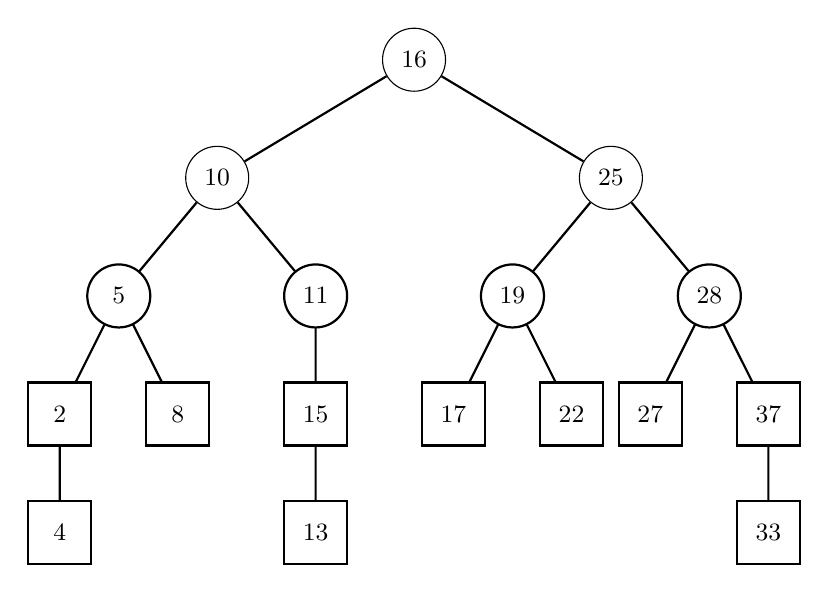
\begin{tikzpicture}[
    % 节点样式定义
    node style/.style={
        circle,              % 圆形节点
        draw,                % 绘制边框
        fill=white,          % 填充白色
        minimum size=0.8cm,  % 最小尺寸
        inner sep=0pt,       % 内部填充为0
        font=\small          % 字体大小
    },
    % 叶子节点样式 (如果需要区分,否则可以都用 node style)
    leaf node style/.style={
        rectangle,           % 方形节点
        draw,
        fill=white,
        minimum size=0.8cm,
        inner sep=2pt,
        font=\small
    },
    % 边样式定义
    edge from parent/.style={
        draw,                % 绘制
        thick                % 粗线
    },
    % 节点间距 (简化,只设置主要层级间距)
    level 1/.style={sibling distance=5cm},
    level 2/.style={sibling distance=2.5cm},
    level 3/.style={sibling distance=1.5cm},
    level 4/.style={sibling distance=0.8cm} % 更细的叶子层间距
]

% 定义节点和树结构
% 根节点
\node[node style] (root) {16}
    % 左子树
    child { node[node style] (node10) {10}
        child { node[node style] (node5) {5}
            child { node[leaf node style] (node2) {2}
                child { node[leaf node style] (node4) {4} } % 2的子节点4
            }
            child { node[leaf node style] (node8) {8} }
        }
        child { node[node style] (node11) {11}
            child { node[leaf node style] (node15) {15} 
                child { node[leaf node style] (node13) {13}
                } % 15的子节点13
            }
        }
    }
    % 右子树
    child { node[node style] (node25) {25}
        child { node[node style] (node19) {19}
            child { node[leaf node style] (node17) {17} }
            child { node[leaf node style] (node22) {22} }
        }
        child { node[node style] (node28) {28}
            child { node[leaf node style] (node27) {27} }
            child { node[leaf node style] (node37) {37}
                child { node[leaf node style] (node33) {33} } % 37的子节点33
            }
        }
    };

\end{tikzpicture}
\\
\begin{solution}
正确答案是 C。
\end{solution}


\section*{101}
\begin{graybox}
对BST进行插入操作,对待插入的目标元素e
进行查找后,若查找失败,\_hot指向的节点为: \\
A. 待插入的节点 \\
B. 被插入后的父亲 \\
C. 被插入后的左孩子 \\
D. 根节点
\end{graybox}

\begin{solution}
正确答案是 B。

\textbf{详细分析:}

在二叉搜索树(BST)的插入操作中,通常会首先执行一个查找操作来确定待插入元素 `e` 的位置。
这个查找过程会从根节点开始,根据 \texttt{e} 与当前节点值的比较,向左或向右子树深入。
变量 \texttt{\_hot} (或者类似名称的变量,如 \texttt{parent} 或 \texttt{p}) 通常用来追踪当前查找路径上节点的父节点。

具体步骤如下:
\begin{enumerate}
    \item 初始化一个指针 \texttt{current} 指向根节点,\texttt{\_hot} 指向 null (或者一个哨兵)。
    \item 当 \texttt{current} 不为 null 时,循环:
    \begin{enumerate}
        \item 将 \texttt{\_hot} 更新为 \texttt{current}。
        \item 如果 \texttt{e} 等于 \texttt{current} 的值,则查找成功(元素已存在,通常不插入或根据策略处理重复)。
        \item 如果 \texttt{e} 小于 \texttt{current} 的值,则 \texttt{current} 移动到其左孩子。
        \item 如果 \texttt{e} 大于 \texttt{current} 的值,则 \texttt{current} 移动到其右孩子。
    \end{enumerate}
    \item 当循环结束时,如果 \texttt{current} 为 null,则表示查找失败。此时,\texttt{\_hot} 指向的是查找路径上最后一个非空节点,也就是新节点 \texttt{e} 应该被插入为其孩子的位置的父节点。
\end{enumerate}

因此,若查找失败,\texttt{\_hot} 指向的节点将成为新插入节点 \texttt{e} 的父亲节点。

分析选项:
\begin{itemize}
    \item \textbf{A. 待插入的节点:} \texttt{\_hot} 指向的是树中已存在的节点,而不是尚未创建的待插入节点。
    \item \textbf{B. 被插入后的父亲:} 这是正确的。\texttt{\_hot} 是查找路径上最后一个访问的非空节点,新节点将作为 \texttt{\_hot} 的左孩子或右孩子插入。
    \item \textbf{C. 被插入后的左孩子:} 新插入的节点是 \texttt{\_hot} 的孩子,而不是 \texttt{\_hot} 是新节点的左孩子。
    \item \textbf{D. 根节点:} 只有当树为空(此时 \texttt{\_hot} 可能为null,新节点成为根)或者新节点直接插入为根节点的子节点时,\texttt{\_hot} 才可能是根节点。一般情况下,\texttt{\_hot} 是查找路径上更深层的节点。
\end{itemize}

所以,\texttt{\_hot} 指向的是被插入节点 \texttt{e} 的父亲节点。
\end{solution}


\section*{102}
\begin{graybox}
当欲删除的节点v在BST中的度为2时,
实际被删除的节点为: \\
A. v在中序遍历下的直接前驱 \\
B. v在先序遍历下的直接后继 \\
C. v的右子树中左侧分支的最后一个节点 \\
D. v的父亲
\end{graybox}

\begin{solution}
正确答案是 C (或者 A,取决于具体实现策略,但C是常见选择)。

\textbf{详细分析:}

当在二叉搜索树(BST)中删除一个度为2的节点 `v`(即 `v` 同时拥有左孩子和右孩子)时,节点 `v` 本身并不会直接从树结构中移除。替代地,采用以下步骤:
\begin{enumerate}
    \item 找到一个替代节点:这个替代节点通常是 `v` 在中序遍历下的直接前驱(即 `v` 左子树中的最大节点)或直接后继(即 `v` 右子树中的最小节点)。
    \item 用替代节点的值替换 `v` 的值。
    \item 然后,删除原来的替代节点。这个替代节点由于其特性(作为子树中的最大或最小元素),其度数最多为1(即它最多只有一个孩子,或者没有孩子),因此删除它会比较简单,可以归约为删除度为0或度为1节点的情况。
\end{enumerate}
所以,“实际被删除的节点”指的是这个被用来替换 `v` 的值的、原来的前驱或后继节点。

现在分析选项:
\begin{itemize}
    \item \textbf{A. v在中序遍历下的直接前驱:}
        这是指 `v` 左子树中的最大节点。如果选择用前驱来替换 `v`,那么这个前驱节点就是实际被从其原位置删除的节点。这是一个有效的策略。

    \item \textbf{B. v在先序遍历下的直接后继:}
        这不是标准BST删除操作中用来替换度为2节点的方法。

    \item \textbf{C. v的右子树中左侧分支的最后一个节点:}
        这描述的是 `v` 在中序遍历下的直接后继,即 `v` 右子树中的最小节点(从右孩子开始,一直向左走到尽头)。如果选择用后继来替换 `v`,那么这个后继节点就是实际被从其原位置删除的节点。这同样是一个有效的、且非常常见的策略。

    \item \textbf{D. v的父亲:}
        `v` 的父亲与此删除过程无关。
\end{itemize}

由于选项 A 和 C 都描述了在标准删除策略中可能被“实际删除”的节点,我们需要判断题目更倾向于哪一个。在许多教材和实现中,选择中序后继(即右子树中的最小节点)作为替代节点是一个非常普遍的做法。

如果必须选择一个,并且考虑到选项 C 对该节点的描述(“v的右子树中左侧分支的最后一个节点”)非常具体地指出了如何找到中序后继,这通常是教学中强调的一个方法。

因此,虽然使用中序前驱(选项 A)也是一种完全正确的策略,但选项 C 描述的中序后继是更常被引用的方法之一。题目问“实际被删除的节点为:”,暗示了一个确定的答案,这通常指向一个标准算法步骤。

假设题目倾向于使用中序后继的策略,则选项 C 是正确的。
\end{solution}


\section*{103}
\begin{graybox}
两个等价的平衡二叉搜索树有相同的: \\
A. 先序遍历序列 \\
B. 中序遍历序列 \\
C. 后序遍历序列 \\
D. 层次遍历序列
\end{graybox}

\begin{solution}
正确答案是 B。

\textbf{详细分析:}

“等价的”平衡二叉搜索树通常指它们包含相同的节点集合(即相同的关键码集合)。
“平衡二叉搜索树”是指满足二叉搜索树性质,并且通过特定算法(如AVL树、红黑树的旋转操作)保持树高在 $O(\log n)$ 数量级的树。

我们来分析各种遍历序列:
\begin{itemize}
    \item \textbf{A. 先序遍历序列 (根-左-右):}
        先序遍历序列与树的具体结构(尤其是根节点和子树的排列)密切相关。即使两棵平衡二叉搜索树包含相同的节点集,它们的具体结构(由于平衡调整的方式或历史操作可能不同)也可能不同,从而导致不同的先序遍历序列。例如,对于节点集 \{1, 2, 3\},一棵平衡树可能是根为2,左孩子1,右孩子3;另一棵(如果允许不同的平衡策略或由不同操作序列形成)可能有不同的根或结构,导致不同的先序序列。

    \item \textbf{B. 中序遍历序列 (左-根-右):}
        对于任何二叉搜索树(无论是否平衡),其中序遍历序列都会得到一个按关键码升序排列的节点序列。如果两棵平衡二叉搜索树是“等价的”(即包含相同的关键码集合),那么它们的中序遍历序列必然是相同的,因为这个序列就是这些关键码的唯一排序结果。
        \textbf{这是正确的。}

    \item \textbf{C. 后序遍历序列 (左-右-根):}
        与先序遍历类似,后序遍历序列也依赖于树的具体结构。不同的平衡结构会导致不同的后序遍历序列。

    \item \textbf{D. 层次遍历序列:}
        层次遍历序列(按层,从左到右)同样高度依赖于树的结构。不同的平衡结构(例如,同一层上的节点顺序或哪些节点在哪些层)会导致不同的层次遍历序列。
\end{itemize}

因此,两个包含相同节点集合的平衡二叉搜索树,它们的中序遍历序列一定是相同的,因为该序列代表了这些节点关键码的有序排列。其他遍历序列则会因树的具体平衡结构不同而可能不同。
\end{solution}



\section*{104}
\begin{graybox}
在AVL树中刚插入一个节点后失衡节点
个数最多为 \\
A. O(1) \\
B. O(loglogn) \\
C. O(logn) \\
D. O(n)
\end{graybox}

\begin{solution}
正确答案是 C。

\textbf{详细分析:}

该问题询问的是在AVL树中插入一个新节点之后、进行任何旋转恢复平衡操作*之前*,树中最多可能有多少个节点的平衡因子变为+2或-2(即“失衡”)。

\begin{enumerate}
    \item \textbf{影响路径:} 插入一个新节点只会影响从该新节点的父节点到根节点这条路径上各个节点的平衡因子。路径外的其他节点的平衡因子不会改变。

    \item \textbf{失衡条件:} 一个节点会变得失衡,当且仅当它的平衡因子原本是+1或-1,并且新节点被插入到了其较高的那个子树中,导致该子树的高度增加了1。

    \item \textbf{最坏情况分析:} 我们可以构造一种情况,使得路径上的多个节点同时满足失衡条件。
    考虑一棵AVL树,其中从根节点到某个叶节点路径上的所有节点,其平衡因子都是-1(或+1)。例如,一条全由左孩子组成的路径,且路径上每个节点的平衡因子都是-1。
    \begin{verbatim}
          p_0 (bf=-1)
         /
        p_1 (bf=-1)
       /
      p_2 (bf=-1)
     /
    ...
    \end{verbatim}
    当一个新的节点被插入到这条路径最末端节点的左子树时:
    \begin{itemize}
        \item 最末端的节点(比如 $p_m$)的左子树高度增加1,其平衡因子从-1变为-2,导致 $p_m$ 失衡。
        \item 由于 $p_m$ 的高度增加了1,这会导致其父节点 $p_{m-1}$ 的左子树高度增加1。因为 $p_{m-1}$ 的平衡因子原本也是-1,所以它现在也变为-2而失衡。
        \item 这个效应会沿着路径一直向上传播。路径上的每一个节点的平衡因子都会从-1变为-2,从而全部失衡。
    \end{itemize}

    \item \textbf{复杂度计算:} 这条路径的最大长度等于AVL树的高度。对于一个包含n个节点的AVL树,其高度为 $O(\log n)$。因此,在最坏情况下,失衡节点的个数可以与树的高度成正比。
\end{enumerate}

所以,在插入一个节点后,失衡节点的个数最多为 $O(\log n)$。

(注:虽然可能会有 $O(\log n)$ 个节点失衡,但AVL树的一个重要特性是,只需要在最靠近插入点的那个失衡节点上执行一次旋转(单旋或双旋),就可以使整棵树恢复平衡。)
\end{solution}



\section*{105}
\begin{graybox}
在AVL树中刚删除一个节点后失衡节点个数
最多为 \\
A. O(1) \\
B. O(loglogn) \\
C. O(logn) \\
D. O(n)
\end{graybox}

\begin{solution}
正确答案是 C。

\textbf{详细分析:}

在AVL树中,删除一个节点比插入一个节点要复杂。删除操作可能导致树的高度降低,这种高度变化会从被删除节点的父节点开始,沿着到根节点的路径向上传播。

\begin{enumerate}
    \item \textbf{影响路径:} 与插入操作类似,删除一个节点只会影响从物理删除点到根节点的路径上各个节点的平衡因子。

    \item \textbf{失衡与传播:}
    与插入操作不同,删除操作后的平衡恢复过程可能不会在第一次旋转后就结束。
    \begin{itemize}
        \item 当一个节点的平衡因子从-1变为0(因其左子树高度降低)或从+1变为0(因其右子树高度降低)时,该节点本身是平衡的,但其所在子树的总高度降低了1。
        \item 这个高度降低会继续向上传播,可能导致其父节点、祖父节点等更高层的节点失衡。
        \item 当这个高度降低的传播最终导致某个祖先节点的平衡因子从+1变为+2或从-1变为-2时,该祖先节点就失衡了。
    \end{itemize}

    \item \textbf{最坏情况:}
    最坏的情况是,高度降低的效应一直传播到根节点。在向上传播的过程中,路径上的每一个节点都可能需要进行检查,并可能需要旋转来恢复平衡。因为在删除后,对一个失衡节点进行旋转,并不能保证其子树的高度恢复到删除前的状态,所以其父节点仍然可能失衡。这个过程需要沿着整条路径一直检查到根。

    \item \textbf{复杂度计算:}
    需要检查和可能需要恢复平衡的节点路径,其最大长度等于AVL树的高度。对于一个包含n个节点的AVL树,其高度为 $O(\log n)$。因此,在删除操作后,沿着路径向上的整个过程中,可能会遇到多个需要调整的失衡节点。
\end{enumerate}

因此,在删除一个节点后,需要考虑进行平衡调整的节点数量(即可能失衡的节点数量)最多可以达到路径的长度,即 $O(\log n)$。
\end{solution}




\section*{106}
\begin{graybox}
AVL树中插入节点引发失衡,经旋转调整后重新平衡,此时包含节点g,p,v的子树高度
\begin{itemize}
\item[A.] 减小1
\item[B.] 不变
\item[C.] 增加1
\item[D.] 有可能不变也有可能增加1
\end{itemize}
\end{graybox}

\begin{solution}
正确答案是 B。

\textbf{详细分析:}

这个问题询问的是,在因插入导致失衡并进行旋转调整后,失衡子树的高度与它在插入操作*之前*的高度相比,发生了什么变化。

\begin{enumerate}
    \item \textbf{插入前的状态:}
    假设失衡发生在以节点 `g` 为根的子树。在插入新节点之前,`g` 是平衡的,我们设其子树高度为 $H$。为了在插入后会失衡,`g` 的平衡因子必须是 +1 或 -1,表示它的一棵子树比另一棵高1。

    \item \textbf{插入后、旋转前的状态:}
    新节点被插入到 `g` 的那棵“更高”的子树中,导致该子树的高度增加了1。这使得 `g` 的两棵子树高度差变为2,`g` 变得失衡。此时,以 `g` 为根的子树的总高度也增加了1,变为 $H+1$。

    \item \textbf{旋转调整后的状态:}
    对以 `g` 为根的失衡子树进行旋转调整(无论是单旋转还是双旋转)。AVL树插入操作后旋转调整的一个关键特性是:\textbf{旋转会使该子树的高度恢复到插入操作之前的原始高度}。
    也就是说,经过旋转后,新的根节点(可能是原来的 `p` 或 `v`)所领导的子树,其高度会变回 $H$。
\end{enumerate}

\textbf{结论:}
\begin{itemize}
    \item 子树在插入前的原始高度为 $H$。
    \item 子树在旋转调整后的高度也是 $H$。
\end{itemize}
因此,与插入操作之前相比,经过“插入-失衡-旋转”这一完整过程后,子树的高度保持不变。
\end{solution}



\section*{107}
\begin{graybox}
经过3+4重构后的AVL树\_\_\_\_\_不变。
A. 先序遍历序列
B. 中序遍历序列
C. 后序遍历序列
D. 层次遍历序列
\end{graybox}

\begin{solution}
正确答案是 B。

\textbf{详细分析:}

“3+4重构”是描述AVL树(以及其他平衡二叉搜索树)旋转操作的一种通用模型。它涉及到三个节点(失衡的祖父节点`g`、其较高的孩子`p`、以及`p`的较高的孩子`v`)和附属于它们的四个可能的子树。

\begin{enumerate}
    \item \textbf{重构的目的:} 旋转或重构操作的根本目的是在不破坏二叉搜索树(BST)基本性质的前提下,恢复树的平衡。

    \item \textbf{BST的基本性质:} 二叉搜索树最重要的性质是,对它进行\textbf{中序遍历}会得到一个所有节点按其关键码升序排列的序列。

    \item \textbf{重构过程:} “3+4重构”通过将`g`, `p`, `v`这三个节点按照它们关键码的大小(a < b < c)重新排列,使得关键码为`b`的节点成为新的子树根,`a`成为其左孩子,`c`成为其右孩子,并重新链接四个子树。这个过程本质上就是一次或两次旋转。

    \item \textbf{不变性分析:}
    \begin{itemize}
        \item \textbf{中序遍历序列:} 由于重构操作必须保持BST的性质,而BST的中序遍历结果是唯一的(即所有元素的排序结果),因此,重构前后子树的中序遍历序列是完全相同的。
        \item \textbf{先序、后序、层次遍历序列:} 这三种遍历方式都与树的具体拓扑结构(谁是根、谁是谁的孩子)密切相关。重构操作改变了`g`, `p`, `v`之间的父子关系,从而改变了树的结构。因此,先序、后序和层次遍历序列几乎总是会发生改变。
    \end{itemize}
\end{enumerate}

\textbf{结论:}
“3+4重构”是一种保持中序遍历序列不变的结构调整。因此,经过重构后,AVL树的中序遍历序列保持不变。
\end{solution}


\section*{108}
\begin{graybox}
AVL树中删除节点引发失衡,经旋转调
整后重新平衡,此时包含节点g,p,v的子树高
度
A. 减小1
B. 不变
C. 增加1
D. 有可能不变也有可能减小1
\end{graybox}

\begin{solution}
正确答案是 D。

\textbf{详细分析:}

在AVL树中,删除操作比插入操作更为复杂,其对高度的影响也不同。当删除一个节点导致以 `g` 为根的子树失衡时,我们需要对 `g` 进行旋转调整。调整后子树的高度变化取决于 `g` 的较高子树(设其根为 `p`)的平衡因子。

\begin{enumerate}
    \item \textbf{失衡的起因:}
    节点 `g` 失衡,是因为它的某一个子树(比如左子树)的高度没有变化,而另一个子树(右子树)因为删除了节点,高度减小了1。这使得 `g` 的平衡因子从-1变为-2(或从+1变为+2)。

    \item \textbf{旋转调整后的高度变化:}
    对 `g` 进行旋转调整后,新的子树高度与 `p` 节点的平衡因子有关:
    \begin{itemize}
        \item \textbf{情况一:如果 `p` 的平衡因子与 `g` 的失衡方向相同} (例如,`g` 是左高,`p` 也是左高,即LL情况),或者相反 (LR情况)。
        在这种情况下,旋转后,整个子树的高度会\textbf{减小1}。由于高度减小,这个变化会继续向上传播,可能导致更高层的祖先节点也失衡。

        \item \textbf{情况二:如果 `p` 的平衡因子为0。}
        在这种情况下,旋转后,整个子树的高度会恢复到删除操作之前的原始高度,即高度\textbf{不变}。由于高度没有变化,平衡调整到此结束,不会再影响更高层的祖先节点。
    \end{itemize}
\end{enumerate}

\textbf{结论:}
与插入操作不同(插入后的旋转总是使子树高度恢复到插入前的高度),删除操作后的旋转调整,可能会使子树高度减小1,也可能使子树高度保持不变。

因此,选项 D “有可能不变也有可能减小1” 是最准确的描述。
\end{solution}


\section*{109}
\begin{graybox}
包含节点\{1,2,3,4\}的不同二叉搜索树有多
少棵?
\end{graybox}

\begin{solution}
答案是 \textbf{14} 棵。

\textbf{详细分析:}

这个问题询问的是,给定 $n$ 个不同的节点,可以构成多少种结构不同的二叉搜索树(BST)。这是一个经典的组合数学问题,其解由第 $n$ 个卡特兰数(Catalan Number)给出。

卡特兰数的计算公式为:
$C_n = \frac{1}{n+1} \binom{2n}{n} = \frac{(2n)!}{(n+1)!n!}$

对于本题,我们有 $n=4$ 个节点。因此,我们需要计算第4个卡特兰数 $C_4$。

$C_4 = \frac{1}{4+1} \binom{2 \times 4}{4} = \frac{1}{5} \binom{8}{4}$

首先计算组合数 $\binom{8}{4}$:
$\binom{8}{4} = \frac{8!}{4!(8-4)!} = \frac{8!}{4!4!} = \frac{8 \times 7 \times 6 \times 5}{4 \times 3 \times 2 \times 1} = \frac{1680}{24} = 70$

然后代入卡特兰数公式:
$C_4 = \frac{1}{5} \times 70 = 14$

\textbf{另一种解释(递归方法):}
令 $C_n$ 为有 $n$ 个节点的BST的数量。
\begin{itemize}
    \item $C_0 = 1$ (空树)
    \item $C_1 = 1$
    \item $C_2 = 2$
    \item $C_3 = 5$
\end{itemize}
我们可以通过选择不同的根节点来构建有4个节点的BST:
\begin{itemize}
    \item \textbf{以1为根:} 左子树有0个节点,右子树有3个节点(\{2,3,4\})。数量 = $C_0 \times C_3 = 1 \times 5 = 5$ 棵。
    \item \textbf{以2为根:} 左子树有1个节点(\{1\}),右子树有2个节点(\{3,4\})。数量 = $C_1 \times C_2 = 1 \times 2 = 2$ 棵。
    \item \textbf{以3为根:} 左子树有2个节点(\{1,2\}),右子树有1个节点(\{4\})。数量 = $C_2 \times C_1 = 2 \times 1 = 2$ 棵。
    \item \textbf{以4为根:} 左子树有3个节点(\{1,2,3\}),右子树有0个节点。数量 = $C_3 \times C_0 = 5 \times 1 = 5$ 棵。
\end{itemize}
总数量 = $5 + 2 + 2 + 5 = 14$ 棵。
\end{solution}


\section*{110}
\begin{graybox}
在以下二叉搜索树中查找元素14,第3个和14发生比较的元素为:
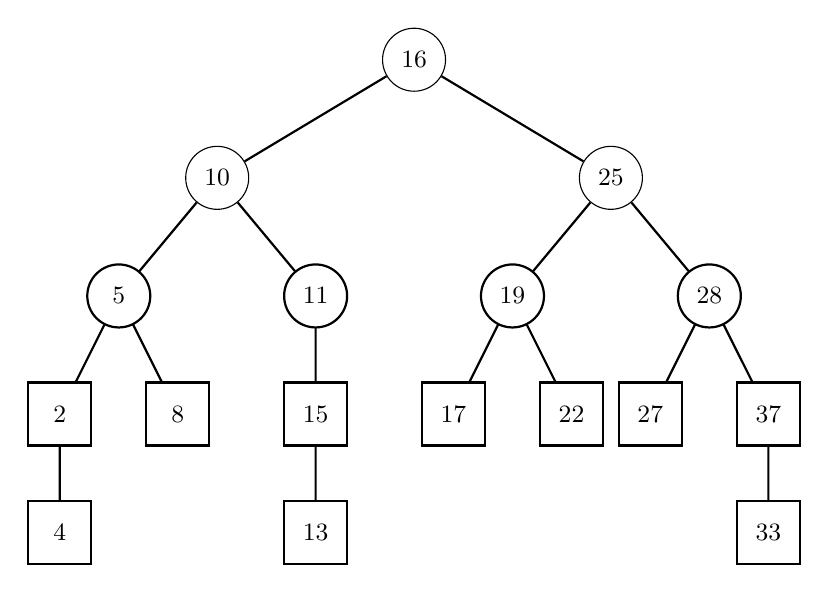
\begin{tikzpicture}[
    % 节点样式定义
    node style/.style={
        circle,              % 圆形节点
        draw,                % 绘制边框
        fill=white,          % 填充白色
        minimum size=0.8cm,  % 最小尺寸
        inner sep=0pt,       % 内部填充为0
        font=\small          % 字体大小
    },
    % 叶子节点样式 (如果需要区分,否则可以都用 node style)
    leaf node style/.style={
        rectangle,           % 方形节点
        draw,
        fill=white,
        minimum size=0.8cm,
        inner sep=2pt,
        font=\small
    },
    % 边样式定义
    edge from parent/.style={
        draw,                % 绘制
        thick                % 粗线
    },
    % 节点间距 (简化,只设置主要层级间距)
    level 1/.style={sibling distance=5cm},
    level 2/.style={sibling distance=2.5cm},
    level 3/.style={sibling distance=1.5cm},
    level 4/.style={sibling distance=0.8cm} % 更细的叶子层间距
]

% 定义节点和树结构
% 根节点
\node[node style] (root) {16}
    % 左子树
    child { node[node style] (node10) {10}
        child { node[node style] (node5) {5}
            child { node[leaf node style] (node2) {2}
                child { node[leaf node style] (node4) {4} } % 2的子节点4
            }
            child { node[leaf node style] (node8) {8} }
        }
        child { node[node style] (node11) {11}
            child { node[leaf node style] (node15) {15} 
                child { node[leaf node style] (node13) {13}
                } % 15的子节点13
            }
        }
    }
    % 右子树
    child { node[node style] (node25) {25}
        child { node[node style] (node19) {19}
            child { node[leaf node style] (node17) {17} }
            child { node[leaf node style] (node22) {22} }
        }
        child { node[node style] (node28) {28}
            child { node[leaf node style] (node27) {27} }
            child { node[leaf node style] (node37) {37}
                child { node[leaf node style] (node33) {33} } % 37的子节点33
            }
        }
    };

\end{tikzpicture}
\\
\end{graybox}

\begin{solution}
答案是 \textbf{11}。

\textbf{详细分析:}
在二叉搜索树中查找元素,我们遵循以下规则:
\begin{itemize}
    \item 如果目标值小于当前节点的值,则移动到左孩子。
    \item 如果目标值大于当前节点的值,则移动到右孩子。
    \item 如果目标值等于当前节点的值,则查找成功。
\end{itemize}

我们来追踪查找元素14的过程:
\begin{enumerate}
    \item \textbf{第1次比较:} 从根节点 \textbf{16} 开始。
        \begin{itemize}
            \item 比较 14 和 16。
            \item 因为 14 < 16,所以向左移动到节点 10。
        \end{itemize}
    \item \textbf{第2次比较:} 当前节点为 \textbf{10}。
        \begin{itemize}
            \item 比较 14 和 10。
            \item 因为 14 > 10,所以向右移动到节点 11。
        \end{itemize}
    \item \textbf{第3次比较:} 当前节点为 \textbf{11}。
        \begin{itemize}
            \item 比较 14 和 11。
            \item 因为 14 > 11,所以继续向右移动。
        \end{itemize}
\end{enumerate}
根据查找路径,第3个与14发生比较的元素是 \textbf{11}。
\end{solution}




\section*{111}
\begin{graybox}
欲在以下二叉搜索树中删除节点16,可行的
方案是:

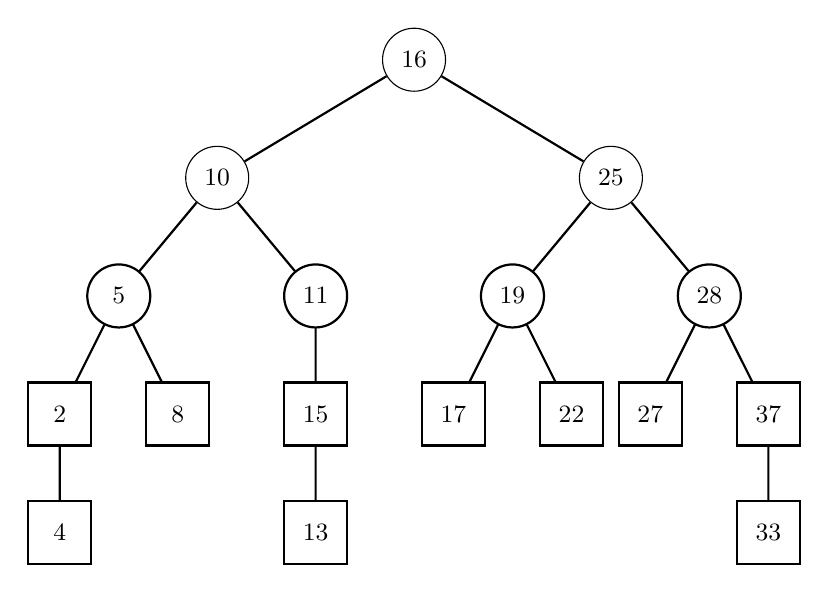
\begin{tikzpicture}[
    % 节点样式定义
    node style/.style={
        circle,              % 圆形节点
        draw,                % 绘制边框
        fill=white,          % 填充白色
        minimum size=0.8cm,  % 最小尺寸
        inner sep=0pt,       % 内部填充为0
        font=\small          % 字体大小
    },
    % 叶子节点样式 (如果需要区分,否则可以都用 node style)
    leaf node style/.style={
        rectangle,           % 方形节点
        draw,
        fill=white,
        minimum size=0.8cm,
        inner sep=2pt,
        font=\small
    },
    % 边样式定义
    edge from parent/.style={
        draw,                % 绘制
        thick                % 粗线
    },
    % 节点间距 (简化,只设置主要层级间距)
    level 1/.style={sibling distance=5cm},
    level 2/.style={sibling distance=2.5cm},
    level 3/.style={sibling distance=1.5cm},
    level 4/.style={sibling distance=0.8cm} % 更细的叶子层间距
]

% 定义节点和树结构
% 根节点
\node[node style] (root) {16}
    % 左子树
    child { node[node style] (node10) {10}
        child { node[node style] (node5) {5}
            child { node[leaf node style] (node2) {2}
                child { node[leaf node style] (node4) {4} } % 2的子节点4
            }
            child { node[leaf node style] (node8) {8} }
        }
        child { node[node style] (node11) {11}
            child { node[leaf node style] (node15) {15} 
                child { node[leaf node style] (node13) {13}
                } % 15的子节点13
            }
        }
    }
    % 右子树
    child { node[node style] (node25) {25}
        child { node[node style] (node19) {19}
            child { node[leaf node style] (node17) {17} }
            child { node[leaf node style] (node22) {22} }
        }
        child { node[node style] (node28) {28}
            child { node[leaf node style] (node27) {27} }
            child { node[leaf node style] (node37) {37}
                child { node[leaf node style] (node33) {33} } % 37的子节点33
            }
        }
    };

\end{tikzpicture}
\\
A. 将16摘除后令25为10的右子,从而10是新的根
节点 \\
B. 以16为轴进行一次zig操作使之不再是根节点,
再直接摘除16 \\
C. 将节点16和节点33的关键码互换,再摘除新的
节点16 \\
D. 将节点16和节点15的关键码互换,摘除新的节
点16并令13为11的右子
\end{graybox}

\begin{solution}
正确答案是 D。

\textbf{详细分析:}

要删除的节点16是根节点,并且它有两个孩子(度为2)。在二叉搜索树(BST)中删除一个度为2的节点,标准算法如下:
\begin{enumerate}
    \item 在该节点的左子树中找到最大的元素(即中序遍历的前驱),或者在其右子树中找到最小的元素(即中序遍历的后继)。
    \item 用找到的这个元素的值替换要删除的节点的值。
    \item 然后,从原位置删除那个被用来替换的节点。由于这个被替换的节点(前驱或后继)最多只有一个孩子,所以删除它会很简单。
\end{enumerate}

我们来分析两种可行的策略:
\begin{itemize}
    \item \textbf{策略1:使用中序前驱}
        \begin{enumerate}
            \item 节点16的中序前驱是其左子树中最大的节点。从左孩子10开始,一直向右走到底,找到节点 \textbf{15}。
            \item 将节点16的值替换为15。
            \item 现在问题变为删除原位置的节点15。这个节点(现在值为16)有一个左孩子13。
            \item 要删除它,我们将其父节点11的右孩子指针指向它的孩子13。即“令13为11的右子”。
        \end{enumerate}
        这个过程与选项D描述的完全一致:“将节点16和节点15的关键码互换,摘除新的节点16并令13为11的右子”。

    \item \textbf{策略2:使用中序后继}
        \begin{enumerate}
            \item 节点16的中序后继是其右子树中最小的节点。从右孩子25开始,一直向左走到底,找到节点 \textbf{17}。
            \item 将节点16的值替换为17。
            \item 现在问题变为删除原位置的节点17。这个节点是叶子节点,可以直接删除。
        \end{enumerate}
\end{itemize}

现在评估所有选项:
\begin{itemize}
    \item A: 这种重构方式会破坏BST的性质,例如19会成为10的后代,但19>10,这不符合规则。
    \item B: Zig操作是伸展树(Splay Tree)中的概念,不是标准BST的删除方法。
    \item C: 节点33既不是16的前驱也不是后继,用它来替换会破坏BST的有序性。
    \item D: 准确描述了使用中序前驱(节点15)来删除节点16的标准过程。
\end{itemize}

因此,选项D是正确的。
\end{solution}



\section*{112}
\begin{graybox}
二叉搜索树的高度h和节点个数n满足关
系
A. h=O(1)
B. h=O(log(n))
C. h=O(n)
D. h=O(nlog(n))
\end{graybox}

\begin{solution}
正确答案是 C。

\textbf{详细分析:}

二叉搜索树(BST)的高度 `h` 与其节点个数 `n` 之间的关系取决于树的平衡程度。我们需要考虑所有可能的情况,特别是最坏情况。

\begin{itemize}
    \item \textbf{最好情况(完全平衡的BST):}
    当二叉搜索树接近完全平衡时,其结构类似于一个完全二叉树。在这种情况下,树的高度 `h` 大约是 $\log_2(n)$。因此,在最好情况下,$h = O(\log n)$。

    \item \textbf{最坏情况(退化的BST):}
    当插入的节点序列是完全有序(升序或降序)时,二叉搜索树会退化成一个线性链表。例如,依次插入 1, 2, 3, ..., n,会形成一个只有右孩子的链。
    \begin{verbatim}
    1
     \
      2
       \
        3
         ...
          \
           n
    \end{verbatim}
    在这种情况下,树的高度为 $n-1$。因此,在最坏情况下,$h = O(n)$。
\end{itemize}

题目询问的是二叉搜索树的一般关系,这必须包含所有情况,尤其是定义其复杂度上界的**最坏情况**。因此,二叉搜索树的高度 `h` 的上界是 $O(n)$。

分析选项:
\begin{itemize}
    \item A. h=O(1): 不正确,高度随节点数增长。
    \item B. h=O(log(n)): 这是平衡二叉搜索树(如AVL树)的高度,是BST的最好情况,但不是所有BST都满足。
    \item C. h=O(n): 这是BST高度的最坏情况,是正确描述其复杂度上界的选项。
    \item D. h=O(nlog(n)): 不正确,这个复杂度与树的高度无关。
\end{itemize}
\end{solution}

\section*{113}
\begin{graybox}
对以下子树进行3+4重构,得到的子树为:
\begin{center}
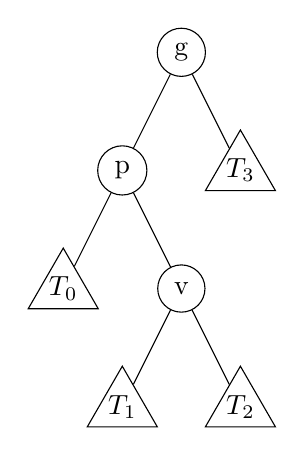
\begin{tikzpicture}[
    node style/.style={circle, draw, fill=white, minimum size=0.6cm},
    subtree style/.style={regular polygon, regular polygon sides=3, draw, minimum size=1cm, inner sep=0pt}
]
\node[node style] (g) {g}
    child { node[node style] (p) {p}
        child { node[subtree style] (T0) {$T_0$} }
        child { node[node style] (v) {v}
            child { node[subtree style] (T1) {$T_1$} }
            child { node[subtree style] (T2) {$T_2$} }
        }
    }
    child { node[subtree style] (T3) {$T_3$} };
\end{tikzpicture}
\end{center}
\end{graybox}

\begin{solution}
\textbf{详细分析:}

“3+4重构”是处理AVL树失衡的一种统一方法。它涉及三个关键节点和四个子树。
\begin{enumerate}
    \item \textbf{识别“3+4”:}
    \begin{itemize}
        \item \textbf{三个节点:} 从最低的失衡节点开始,向上追溯三代:失衡节点 `g` (grandparent),其较高的孩子 `p` (parent),以及 `p` 的较高的孩子 `v` (vulnerable)。
        \item \textbf{四个子树:} 这三个节点将整棵子树分割成四个部分,我们按中序遍历的顺序列出它们:$T_0, T_1, T_2, T_3$。
    \end{itemize}
    根据题目给出的图,我们可以识别出:
    \begin{itemize}
        \item 三个节点是:`g`, `p`, `v`。
        \item 四个子树是:`p`的左子树 $T_0$,`v`的左子树 $T_1$,`v`的右子树 $T_2$,以及`g`的右子树 $T_3$。
    \end{itemize}

    \item \textbf{确定中序次序:}
    对这三个节点进行中序排序。根据二叉搜索树的性质,中序遍历序列为:...$T_0$... \textbf{p} ...$T_1$... \textbf{v} ...$T_2$... \textbf{g} ...$T_3$...
    因此,这三个节点的有序序列是 `p`, `v`, `g`。

    \item \textbf{进行重构:}
    \begin{itemize}
        \item 将有序序列中的中间节点 `v` 提升为新的根。
        \item 将序列中的第一个节点 `p` 作为新根 `v` 的左孩子。
        \item 将序列中的第三个节点 `g` 作为新根 `v` 的右孩子。
        \item 将四个子树 $T_0, T_1, T_2, T_3$ 按照中序次序重新链接到 `p` 和 `g` 上。
            \begin{itemize}
                \item $T_0$ 链接为 `p` 的左孩子。
                \item $T_1$ 链接为 `p` 的右孩子。
                \item $T_2$ 链接为 `g` 的左孩子。
                \item $T_3$ 链接为 `g` 的右孩子。
            \end{itemize}
    \end{itemize}
\end{enumerate}

\textbf{重构后的子树结构为:}
\begin{center}
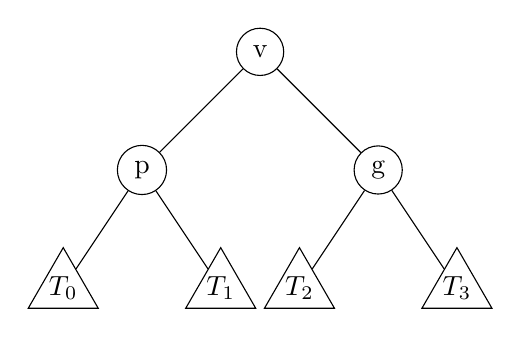
\begin{tikzpicture}[
    node style/.style={circle, draw, fill=white, minimum size=0.6cm},
    subtree style/.style={regular polygon, regular polygon sides=3, draw, minimum size=1cm, inner sep=0pt},
    level 1/.style={sibling distance=3cm},
    level 2/.style={sibling distance=2cm}
]
\node[node style] (v) {v}
    child { node[node style] (p) {p}
        child { node[subtree style] (T0) {$T_0$} }
        child { node[subtree style] (T1) {$T_1$} }
    }
    child { node[node style] (g) {g}
        child { node[subtree style] (T2) {$T_2$} }
        child { node[subtree style] (T3) {$T_3$} }
    };
\end{tikzpicture}
\end{center}
\end{solution}




\end{document}

% VScode 常用快捷键:

% Ctrl + R:                 打开最近的文件夹
% F2:                       变量重命名
% Ctrl + Enter:             行中换行
% Alt + up/down:            上下移行
% 鼠标中键 + 移动:           快速多光标
% Shift + Alt + up/down:    上下复制
% Ctrl + left/right:        左右跳单词
% Ctrl + Backspace/Delete:  左右删单词    
% Shift + Delete:           删除此行
% Ctrl + J:                 打开 VScode 下栏(输出栏)
% Ctrl + B:                 打开 VScode 左栏(目录栏)
% Ctrl + `:                 打开 VScode 终端栏
% Ctrl + 0:                 定位文件
% Ctrl + Tab:               切换已打开的文件(切标签)
% Ctrl + Shift + P:         打开全局命令(设置)

% Latex 常用快捷键

% Ctrl + Alt + J:           由代码定位到PDF
% 


% Git提交规范:
% update: Linear Algebra 2 notes
% add: Linear Algebra 2 notes
% import: Linear Algebra 2 notes
% delete: Linear Algebra 2 notes
